\documentclass[10pt]{article}
\usepackage[a4paper,margin=.72in,headheight=15pt]{geometry}
\usepackage[T1]{fontenc}\usepackage[utf8]{inputenc}\usepackage{lmodern,microtype,amsmath,amssymb,graphicx,xcolor,booktabs,tabularx,hyperref,fancyhdr}
\definecolor{ink}{HTML}{153F50}\definecolor{accent}{HTML}{0072B2}
\setlength{\parindent}{0pt}\setlength{\parskip}{7pt}\setlength{\emergencystretch}{3em}
\hypersetup{colorlinks=true,urlcolor=accent}
\pagestyle{fancy}\fancyhf{}\fancyhead[L]{\small\color{ink}GLOVER | INDEPENDENT RESEARCH WHITE PAPER}\fancyhead[R]{\small 2026}\fancyfoot[C]{\thepage}
\begin{document}

{\small\color{accent}Research argument}\par
{\LARGE\bfseries\color{ink}Drugs Are Good: An Allopath's Journey Through Medicine, Healing, and Danger}\par\vspace{7pt}
Michael Emanuel Glover\par Developed in dialogue with Codex | 4 October 2026\par\vspace{8pt}
I want medicine to succeed. I want suffering relieved, diseases treated and the ordinary pleasures of being alive returned to people whose days have become a struggle. Drugs are good when they do that work well. The title is a declaration of interest in healing, and the rest of the sentence matters: medicine, healing and danger belong in the same inquiry.\par
I approach this journey as an independent author examining the logic of medicine. Allopath names the orientation toward testable treatment in this essay; it does not assert a medical qualification. I do not invent a professional biography, a clinical practice or a series of patients to lend the argument authority. The argument must earn its authority through clear questions, explicit assumptions and evidence.\par
My project combines a first-person account of what I want from medicine with mathematical propositions about simplified exposure and response. Eight color figures make the assumptions visible. Every numerical compound, response parameter and population in these experiments is fictional. The calculations establish consequences of their stated models; they do not establish the safety or efficacy of an actual medicine.\par
There is room for enthusiasm and exactness in the same sentence. I will name what has been measured, what has been assumed and what would have to happen before a simulation could bear clinical weight. Let healing be the aim and scrutiny be part of the work. Selah.\par
\clearpage
{\small\color{accent}Research argument}\par
{\LARGE\bfseries\color{ink}Abstract: the claim and its conditions}\par\vspace{7pt}
I formulate a conditional account of medicinal benefit. A treatment claim specifies a target population, an intervention, a comparator, an outcome and a time horizon. Changing any of these can change what the claim means. The numerical part develops a dimensionless one-compartment exposure model, saturating response functions, value-dependent utility, population heterogeneity and a binomial bound for unobserved rare events.\par
The analytic results are elementary but consequential: positive initial exposure decays under positive first-order elimination; area under the concentration curve is inversely proportional to elimination rate under fixed initial concentration; Hill response remains bounded; a fixed relative event reduction produces different absolute benefits at different baseline risks; and observing no events leaves a positive upper bound on event probability.\par
These results clarify why a compound cannot be evaluated solely by its name or a single attractive response curve. The proposition that medicines can heal is compatible with the proposition that a particular treatment can harm a particular person. Identifying which circumstances apply requires empirical work that this mathematical essay does not substitute for.\par
The completed contribution is a reproducible conceptual and numerical white paper. It includes no patient records, actual treatment schedules, disease-specific parameter estimates or personal prescribing recommendations. The sources provide regulatory context; the calculations supply examples of reasoning, not a clinical decision tool.\par
\clearpage
{\small\color{accent}Research argument}\par
{\LARGE\bfseries\color{ink}A journey through questions rather than invented patients}\par\vspace{7pt}
A journey can be intellectual without being fictitiously autobiographical. My starting point is the attraction of intervention: something is wrong, a material process can be altered, and a person might be helped. The next step is a harder question. What observation would show that the intervention caused the improvement rather than merely preceded it?\par
A person can improve after receiving a treatment because the treatment worked, because the condition fluctuated, because another intervention mattered, or because the initial observation was unusually severe. An account that admits only the first explanation mistakes sequence for proof. An account that never allows the first explanation mistakes skepticism for a conclusion.\par
I want an inquiry capable of revising its expectations in either direction. A theory that predicts benefit should specify the observations under which confidence falls. A theory that predicts harm should permit well-conducted evidence to establish benefit in a defined setting. The discipline is to keep the conclusion responsive to what actually happens.\par
This is the first connection to my broader axiomatic work. A formal system makes implications inspectable; empirical medicine asks whether the premises, measurement process and scope describe the people to whom the result will be applied. The proof and the observation do different jobs, and both jobs matter.\par
\clearpage
{\small\color{accent}Research argument}\par
{\LARGE\bfseries\color{ink}Primitives: person, intervention, outcome, time}\par\vspace{7pt}
I begin with a person index, a time index, an intervention variable and an outcome variable. These are formal placeholders, not complete accounts of a life. An outcome could represent a measured symptom, a laboratory quantity, survival within a defined interval or a patient-reported ability to participate in ordinary activity. Each choice needs a measurement rule.\par
An intervention includes more than the identity of a substance. Its formulation, delivery, exposure history and surrounding care can matter to the question being studied. A comparator can be another treatment, a placebo or a specified care pathway. Calling the comparator 'nothing' usually hides decisions about what actually occurs in that group.\par
Benefit and harm are relational descriptions of changes in outcomes under a stated comparison. I reserve these words for endpoints that have been named. A reduction in one undesirable outcome does not automatically establish improvement in every other outcome. A measurement with an impressive scale does not become important merely because it is easy to collect.\par
The mathematical primitive is deliberately modest: an unknown relation among intervention, state and observation. I will construct examples of such relations, then ask which parts are identifiable from data. That avoids making a person's full experience a single number by definition.\par
\[i\in\mathcal I,\quad t\in[0,T],\quad a\in\mathcal A,\quad Y_i(t;a)\in\mathcal Y.\]
\clearpage
{\small\color{accent}Research argument}\par
{\LARGE\bfseries\color{ink}Axioms of the illustrative exposure model}\par\vspace{7pt}
Axiom E1 states that the illustrative concentration is nonnegative and dimensionless. Axiom E2 states that, after the chosen initial time, the system has one well-mixed compartment and no further input. Axiom E3 states that elimination is proportional to current concentration with a strictly positive constant. These are assumptions of an invented system.\par
Axiom E4 fixes the initial concentration. Axiom E5 treats the observation as an exact reading of that concentration until uncertainty is introduced explicitly. These assumptions allow a short closed-form solution. They do not follow from the title of the paper, and they do not describe every substance or route of administration.\par
The word compartment is a modeling abstraction. It does not assert that the human body consists of one homogeneous vessel. If distribution, delayed input, changing elimination or multiple interacting compartments are necessary for a real research question, this model must be replaced or extended before its predictions can be assessed.\par
I choose a simple system because its consequences can be checked directly. The virtue is inspectability: any numerical error can be compared with a known analytic solution. A transparent model provides a baseline for understanding complexity, provided its simplicity remains visible.\par
\[\dot C(t)=-kC(t),\quad C(0)=C_0\geq0,\quad k>0.\]
\clearpage
{\small\color{accent}Research argument}\par
{\LARGE\bfseries\color{ink}Theorem E1: positivity and exponential decay}\par\vspace{7pt}
Theorem E1. Under E1-E4, the unique solution is the initial concentration multiplied by an exponential decay factor. It remains nonnegative. If the initial concentration is positive, it decreases strictly and tends to zero as time increases without bound. If the initial concentration is zero, it remains zero.\par
Proof. Multiply the differential equation by the integrating factor exp(kt). The derivative of the product is zero, so the product equals its initial value. Rearrangement gives the stated solution. Positivity follows because the exponential is positive; monotonicity follows from the sign of the derivative; the limit follows from positive k.\par
The plot compares three invented elimination constants with the same initial concentration. Its horizontal and vertical axes have no clinical units. A slower decay retains more exposure within this model. The plot makes no statement about whether that extra exposure would help or harm a person.\par
This distinction will recur. A theorem about concentration is a theorem about concentration. To infer an outcome, one needs a response model; to infer an actual human outcome, one needs evidence supporting that response model. Each bridge adds assumptions and opportunities for error.\par
\[C(t)=C_0e^{-kt},\qquad \lim_{t\to\infty}C(t)=0.\]
\begin{center}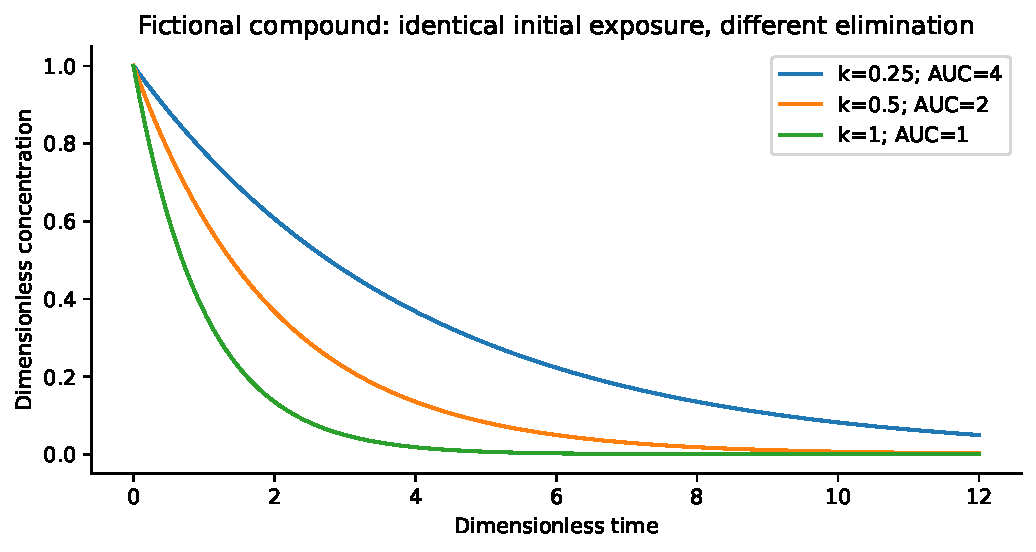
\includegraphics[width=.97\linewidth,height=.26\textheight,keepaspectratio]{figures/elimination.pdf}\end{center}
{\footnotesize Synthetic dimensionless trajectories; all three curves begin at C0=1. No drug or patient is represented.\par}
\clearpage
{\small\color{accent}Research argument}\par
{\LARGE\bfseries\color{ink}Theorem E2: area and half-life}\par\vspace{7pt}
Theorem E2. The integral of concentration over all nonnegative time equals initial concentration divided by the positive elimination constant. For positive initial concentration, the time required for concentration to halve equals the natural logarithm of two divided by that constant.\par
Proof. Integrating the exponential solution yields a finite integral because k is positive. For the half-life, equate the solution to one half of the initial concentration, divide by the positive initial value and take logarithms. The numerical experiment independently integrates the curve and verifies both identities.\par
For k equal to 0.25, 0.5 and 1 with initial concentration one, the dimensionless areas are respectively 4, 2 and 1. Their half-lives are about 2.773, 1.386 and 0.693. These values belong solely to the invented system. They are not estimates for an unnamed medicine.\par
An area summarizes exposure while discarding its temporal shape. Two curves can have the same integral and different peaks or durations above a response threshold. The theorem therefore supplies an exposure identity, not a universal sufficient statistic for benefit or danger.\par
\[\mathrm{AUC}=\int_0^\infty C(t)\,dt=\frac{C_0}{k},\qquad t_{1/2}=\frac{\log2}{k}.\]
\clearpage
{\small\color{accent}Research argument}\par
{\LARGE\bfseries\color{ink}Response: a bounded function is not a clinical endpoint}\par\vspace{7pt}
I introduce a Hill function with a positive scale parameter and positive exponent. It is a convenient example of a saturating response: zero input gives zero response, increasing input increases response, and the limiting response is one. This is a mathematical family chosen for illustration, not a finding that all clinical effects follow this shape.\par
Theorem R1. For nonnegative concentration, the Hill response lies between zero and one. For positive concentration its derivative is positive, and the scale parameter marks the point where response equals one half. Proof follows by comparing numerator and denominator and differentiating the quotient.\par
The figure chooses different scales and exponents for two fictional responses labeled benefit and harm. Those labels give the example a purpose; they do not validate a measurement. The difference curve uses equal weights by convention. A real comparison would need endpoint definitions, estimates, uncertainty and a reason for the chosen weighting.\par
Saturation also means that more exposure can produce progressively less additional response. It says nothing, by itself, about the complete consequences of increasing exposure. A second response can have a different shape, and a person can experience effects absent from both curves.\par
\[H(C;K,n)=\frac{C^n}{K^n+C^n},\quad K,n>0,\quad H(K;K,n)=\frac12.\]
\begin{center}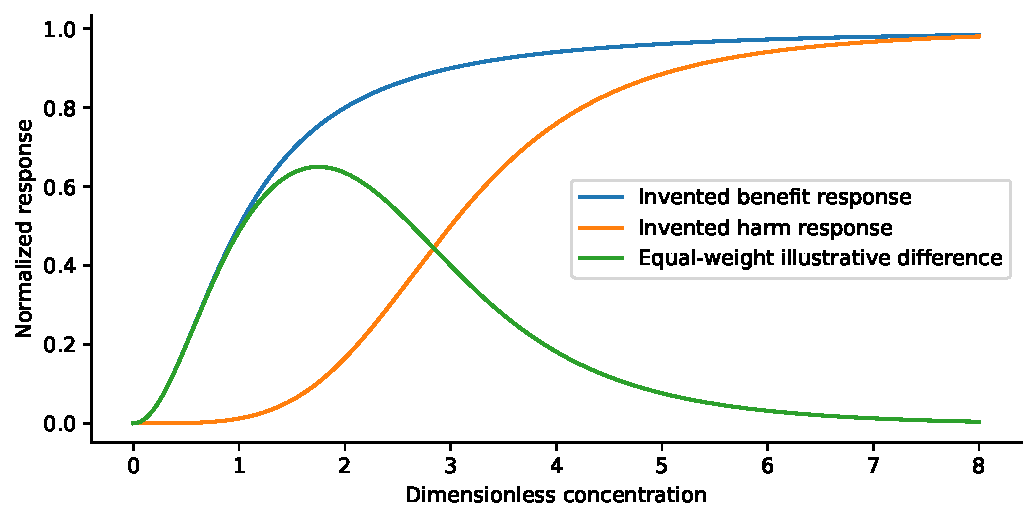
\includegraphics[width=.97\linewidth,height=.26\textheight,keepaspectratio]{figures/responses.pdf}\end{center}
{\footnotesize Invented benefit B=C-squared/(1+C-squared) and harm H=C-to-the-fourth/(81+C-to-the-fourth); labels are illustrative, not measured outcomes.\par}
\clearpage
{\small\color{accent}Research argument}\par
{\LARGE\bfseries\color{ink}An optimum is conditional on an objective}\par\vspace{7pt}
Define a toy utility as the benefit response minus a positive weight times the harm response. Concentration is restricted to a compact interval. Because both response functions are continuous, the utility is continuous and attains a maximum on that interval. This existence theorem does not assert uniqueness or clinical suitability.\par
Proof of existence. The interval is closed and bounded; continuous real-valued functions on such an interval attain their extrema. If the interval, response functions or weight change, the maximizer can change. Even perfect arithmetic cannot decide which human values should enter the objective.\par
The surface displays the invented utility against concentration and harm weight. It shows how an apparently best point depends on a value choice. A claimed universal optimum that omits its weight has hidden part of the question. A claimed optimum without uncertainty has hidden another part.\par
I want algorithms that make these dependencies visible. In a real treatment study, selecting an objective would require meaningful patient participation and clinical judgment, alongside evidence about effects. Here the objective is used to examine an elementary principle: optimizing a function does not establish that the function expresses the right goal.\par
\[U_w(C)=B(C)-wH(C),\quad w>0,\quad C\in[0,8].\]
\begin{center}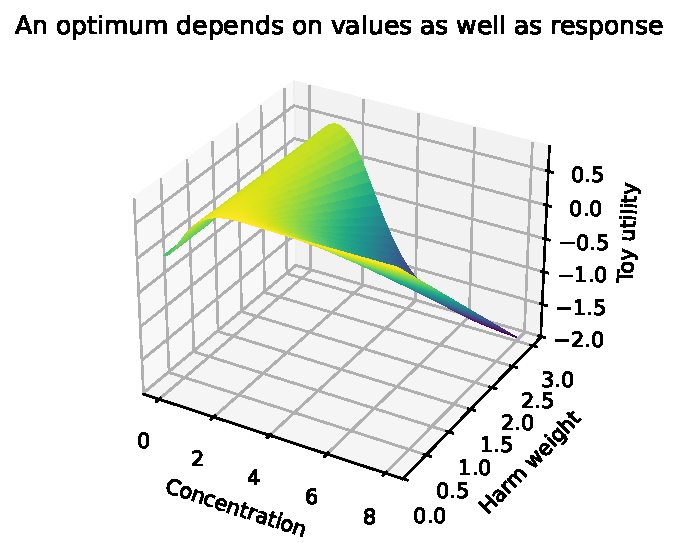
\includegraphics[width=.97\linewidth,height=.26\textheight,keepaspectratio]{figures/utility-surface.pdf}\end{center}
{\footnotesize Three-dimensional synthetic utility surface. Concentration and weights have no prescribing interpretation.\par}
\clearpage
{\small\color{accent}Research argument}\par
{\LARGE\bfseries\color{ink}Grid search and the limits of numerical authority}\par\vspace{7pt}
The experiment evaluates the toy utility on a fixed concentration grid and records the maximizing grid location for each harm weight. The result is reproducible and conditional on that grid. A discrete maximizer is not automatically the exact maximizer of the continuous function.\par
For a continuous objective on a compact interval, refining a uniform grid makes the grid maximum value approach the continuous maximum value. Uniform continuity supplies the proof: every true maximizer has a nearby grid point whose function value differs arbitrarily little once the mesh is sufficiently fine. Convergence of the selected location additionally requires care when several maxima exist.\par
The step-like features in the graph partly reflect grid resolution. They should not be interpreted as a biological switch. This is a useful caution when colorful numerical output acquires more apparent precision than the underlying calculation supports.\par
A numerical optimum also inherits every misspecification in its objective. Refinement can reduce discretization error while leaving model error untouched. I therefore distinguish arithmetic accuracy, mathematical convergence, empirical calibration and the appropriateness of the decision criterion. None of these replaces the others.\par
\begin{center}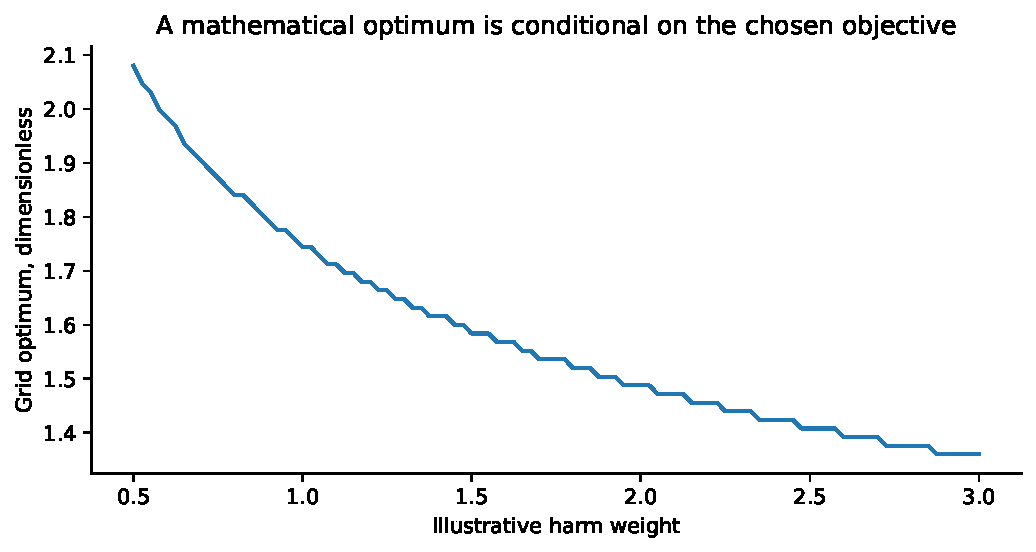
\includegraphics[width=.97\linewidth,height=.26\textheight,keepaspectratio]{figures/optima.pdf}\end{center}
{\footnotesize Synthetic grid maximizers as the harm weight changes; this is a sensitivity illustration, not an actionable exposure target.\par}
\clearpage
{\small\color{accent}Research argument}\par
{\LARGE\bfseries\color{ink}Heterogeneity: a population does not equal its median}\par\vspace{7pt}
The next experiment replaces a common elimination constant with invented positive values drawn from a lognormal distribution. All simulated individuals still begin with concentration one. The random seed is fixed, and the distribution has been selected for demonstration rather than estimated from people.\par
The plot displays pointwise fifth, fiftieth and ninety-fifth percentiles of concentration. These are summaries across simulated individuals at each time. The shaded area is not a confidence interval for an estimated mean, and it is not a guarantee that a particular individual's entire trajectory will remain inside it.\par
The median trajectory is a useful visual summary, but it conceals differences in exposure. This model provides an especially simple example: every individual's area equals the reciprocal of their own elimination constant. Substituting the average constant into that formula generally does not reproduce the average area.\par
For a positive random constant with finite reciprocal expectation, convexity gives the mean reciprocal at least as large as the reciprocal mean. Equality holds for a constant distribution. The conclusion concerns averaging a nonlinear function; its clinical relevance would depend on whether the distribution and model actually described a population.\par
\[\mathbb E[1/K]\geq1/\mathbb E[K],\quad K>0,\]
\begin{center}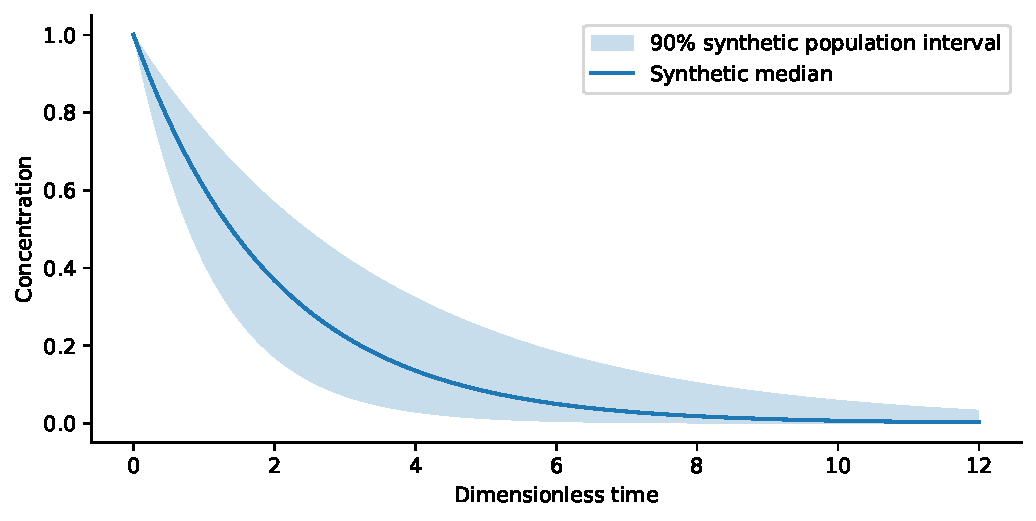
\includegraphics[width=.97\linewidth,height=.26\textheight,keepaspectratio]{figures/uncertainty.pdf}\end{center}
{\footnotesize 20,000 synthetic individuals; log K has mean log(0.5) and standard deviation 0.35. Pointwise population quantiles are shown.\par}
\clearpage
{\small\color{accent}Research argument}\par
{\LARGE\bfseries\color{ink}Interactions: a change in the system can change the answer}\par\vspace{7pt}
Within the toy exposure model, replacing k by half of k doubles area under the curve at the same initial concentration. This is an algebraic consequence of the area identity. It is not a forecast for any actual combination of medicines, and it does not capture changes in response unrelated to concentration.\par
FDA consumer guidance describes interactions involving other medicines, foods or beverages, and existing conditions. It explains that interactions can alter effects or produce harm and emphasizes reviewing labels and discussing the complete medication and supplement list with clinicians or pharmacists [2]. This supplies practical context for why a treatment should not be considered in isolation.\par
A complete interaction model might modify input, distribution, elimination, response or several of these at once. A single parameter change is a teaching device. It would be a mistake to interpret every interaction as slower clearance or to infer its direction from this particular illustration.\par
For research, I would record the proposed mechanism, observable implications and alternative explanations separately. The question is not whether a graph looks plausible. It is whether a sufficiently specific prediction survives measurement in the relevant setting.\par
\[\frac{\mathrm{AUC}(k/2)}{\mathrm{AUC}(k)}=2\quad\text{for fixed }C_0>0.\]
\clearpage
{\small\color{accent}Research argument}\par
{\LARGE\bfseries\color{ink}Relative effects and absolute consequences}\par\vspace{7pt}
Suppose an entirely fictional intervention reduces a defined event probability by a fixed relative fraction. The absolute reduction equals that fraction multiplied by the untreated event probability. The same relative effect therefore produces different absolute differences when the initial probabilities differ.\par
For illustration, a 25\% relative reduction changes a probability of 0.20 to 0.15, an absolute difference of 0.05. The same fraction changes 0.02 to 0.015, an absolute difference of 0.005. Neither example comes from a study of a medicine. Their purpose is to make the denominator visible.\par
Where a causal absolute reduction is positive and appropriately estimated, its reciprocal is often expressed as a number needed to treat over the stated horizon. That summary inherits the population, endpoint and horizon of the underlying comparison. An inverse near zero is unstable, and benefit and harm require separate endpoints rather than casual subtraction of unrelated counts.\par
A percentage stripped of its starting risk can sound decisive while leaving the practical question unresolved. I want the reporting to give both scales, with uncertainty, so that a reader can understand the size of the change and the population to which it refers.\par
\[p_1=(1-r)p_0,\quad\mathrm{ARR}=rp_0,\quad \mathrm{NNT}=1/\mathrm{ARR}\;(\mathrm{ARR}>0).\]
\begin{center}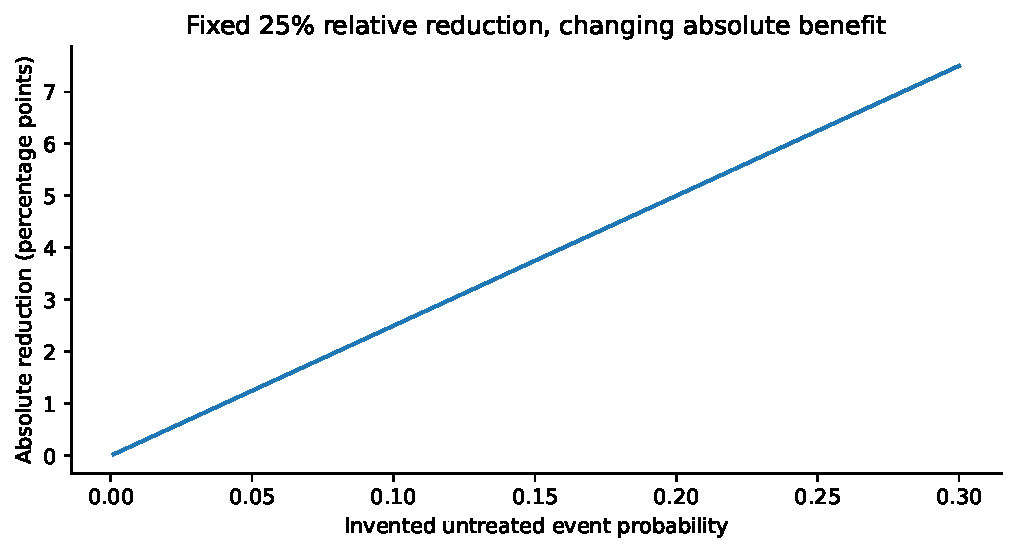
\includegraphics[width=.97\linewidth,height=.26\textheight,keepaspectratio]{figures/absolute-benefit.pdf}\end{center}
{\footnotesize Invented fixed relative reduction r=0.25; absolute benefit changes with the assumed untreated probability.\par}
\clearpage
{\small\color{accent}Research argument}\par
{\LARGE\bfseries\color{ink}Counterfactuals: what would have happened otherwise?}\par\vspace{7pt}
Write an outcome under treatment and an outcome under a specified comparator for each individual. Their difference defines an individual causal contrast within the notation. An individual usually contributes only the outcome under the intervention actually received; the other outcome is counterfactual.\par
An average causal contrast is a population quantity. Observed differences between treated and untreated people need not equal it, because the groups may differ before intervention. The formal notation makes the missing comparison visible without solving it.\par
Random allocation can support identification of a treatment-assignment effect when its design and analysis are respected. Attrition, outcome measurement, deviations from assignment and selective reporting still require attention. A causal claim needs an estimand: the effect of assignment, exposure or adherence can be different questions.\par
This section is a methodological argument, not a claim that a particular trial has succeeded. My numerical exposure examples do not contain random treatment assignment or outcomes from real people. No causal human effect is estimated in this paper. That distinction prevents the mathematical apparatus from lending an unsupported interpretation to synthetic data.\par
\[\mathrm{ATE}=\mathbb E[Y(1)-Y(0)].\]
\clearpage
{\small\color{accent}Research argument}\par
{\LARGE\bfseries\color{ink}From discovery to evidence}\par\vspace{7pt}
FDA describes drug development through discovery, preclinical research, clinical research, regulatory review and monitoring after products reach the market [1]. That sequence is useful context for this essay: a mechanism, a simulation and an observed human outcome occupy different evidentiary positions.\par
My equations begin near the mechanism end of that sequence. They specify what happens if a simplified system behaves as assumed. They do not supply toxicology, patient outcomes, manufacturing evaluation or evidence for an indication. A mathematically elegant model remains a research contribution of a particular kind.\par
The intellectual temptation is to treat a missing stage as a formality once a model feels compelling. I resist that temptation because the missing observation is often precisely where the conclusion could change. An intervention can match a narrow mechanism and fail on an outcome that matters to people.\par
I also distinguish failure of a hypothesis from failure of inquiry. A well-designed study that overturns a plausible claim has increased knowledge. The goal is not to protect a favored equation from reality; the goal is to learn which interventions achieve the desired result under identifiable conditions.\par
{\small [1] FDA. The Drug Development Process. Accessed 4 October 2026.\par\url{https://www.fda.gov/patients/learn-about-drug-and-device-approvals/drug-development-process}\par}
\clearpage
{\small\color{accent}Research argument}\par
{\LARGE\bfseries\color{ink}Theorem S1: zero observed events does not prove zero risk}\par\vspace{7pt}
Consider n independent observations with the same unknown event probability p. The probability of observing no events is the nth power of one minus p. Solving for the probability at which this zero-event observation has probability 0.05 gives an exact one-sided 95\% binomial upper confidence bound when the observed count is zero.\par
At n equal to 1,000, the bound is approximately 0.002991. Its large-sample approximation is about three divided by n. The calculation is an illustration of limited information, not a safety estimate for a drug. Independence, a common probability and a consistently observed event are required assumptions.\par
The confidence level is a repeated-sampling property of a procedure. It is not the probability that an unknown fixed parameter lies below this particular bound after the data have been observed. A Bayesian probability statement would additionally specify a prior and update it.\par
No observed harm is encouraging evidence in a suitably designed study, but it is not a proof that harm cannot occur. The theorem supplies a quantitative reason to keep that distinction. If events are missed or people are dependent, the binomial calculation may be inappropriate even as an uncertainty summary.\par
\[P(X=0\mid p)=(1-p)^n,\qquad p_U=1-0.05^{1/n}.\]
\begin{center}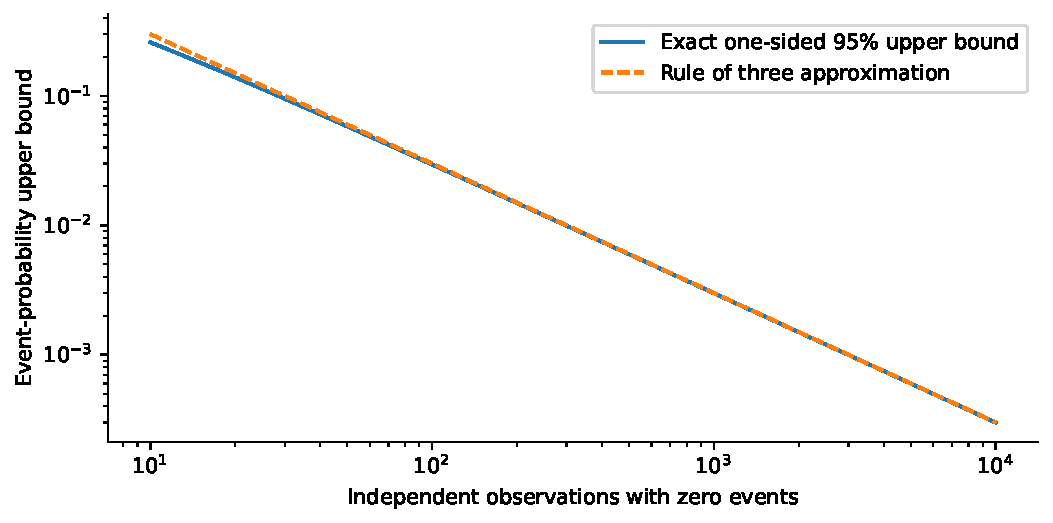
\includegraphics[width=.97\linewidth,height=.26\textheight,keepaspectratio]{figures/zero-events.pdf}\end{center}
{\footnotesize Exact zero-event binomial bound and the 3/n approximation; no real safety observations are included.\par}
\clearpage
{\small\color{accent}Research argument}\par
{\LARGE\bfseries\color{ink}Bayesian updating and the cost of certainty}\par\vspace{7pt}
Bayesian notation gives a second way to express learning about an unknown event probability. A beta prior combined with binomial counts produces a beta posterior whose parameters add observed events and non-events to the prior parameters. This is an exact result under the assumed likelihood and prior.\par
The choice of prior matters, especially when data are sparse. Calling it a prior does not make it arbitrary in every respect: it can be justified, challenged and varied in sensitivity analyses. Calling the posterior a probability does not remove dependence on the model of how observations were generated.\par
I would report how important conclusions change under plausible alternative priors and measurement assumptions. If the answer reverses under small changes, that sensitivity is part of the result. It should not be hidden behind a single polished number.\par
The relation to my axiomatic project is direct. Proof can establish the update rule after assumptions are fixed; empirical judgment must assess those assumptions and the relevance of the data. Confidence that outruns these conditions becomes a rhetorical effect rather than an earned consequence of analysis.\par
\[p\sim\mathrm{Beta}(a,b),\quad X\mid p\sim\mathrm{Binomial}(n,p),\]
\[p\mid X=x\sim\mathrm{Beta}(a+x,b+n-x),\qquad a,b>0.\]
\clearpage
{\small\color{accent}Research argument}\par
{\LARGE\bfseries\color{ink}Numerical verification: compute, compare, disclose}\par\vspace{7pt}
The experiment uses an analytic differential equation precisely so that the implementation can be checked. Numerical integration reproduces the exact area for each selected elimination constant. Evaluation at each analytic half-life returns one half of the starting concentration. Response functions remain inside their prescribed bounds.\par
A separate forward-Euler calculation approximates concentration at dimensionless time four with successive time steps. For the chosen positive constant, the endpoint error decreases as the step decreases. This checks the intended first-order numerical behavior in this example; it does not validate a biological mechanism.\par
The seeded population calculation also checks ordering of the reported quantiles. All parameter values, the seed and results are written to a machine-readable file. Plots can be regenerated without retrieving patient information or contacting an external service.\par
Verification asks whether the code solves the equations as intended. Validation asks whether the equations describe a relevant part of the world. The first can succeed while the second remains unattempted. My report makes that status explicit because a correct computation deserves a precise description of what it has computed.\par
\begin{center}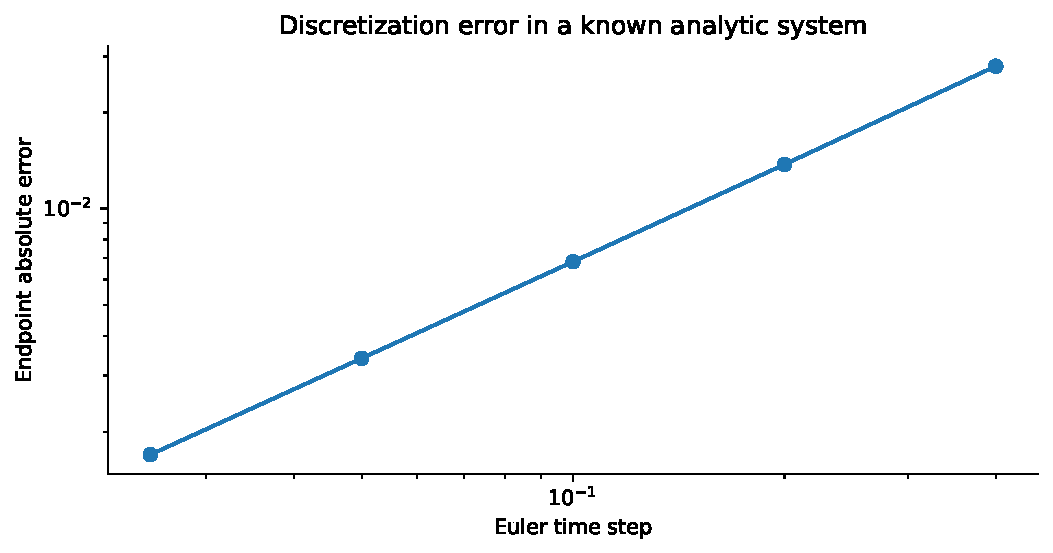
\includegraphics[width=.97\linewidth,height=.26\textheight,keepaspectratio]{figures/convergence.pdf}\end{center}
{\footnotesize Forward Euler at final time 4 with k=0.5 and C0=1; step refinement is checked against exp(-2).\par}
\clearpage
{\small\color{accent}Research argument}\par
{\LARGE\bfseries\color{ink}Results ledger: what the calculations actually establish}\par\vspace{7pt}
The table records analytic quantities and one statistical bound. These are completed results from the specified illustrative systems. There is no invented clinical cohort hidden behind them and no attempt to portray synthetic outcomes as measured patient responses.\par
The utility calculation further identifies a maximizing point on its fixed grid. That location is conditional on the selected benefit and harm functions, equal weighting and the grid resolution. It is stored for reproducibility rather than proposed as a treatment target.\par
The population result describes variability under an invented lognormal distribution. A different distribution would generate different quantiles and exposure summaries. The appropriate empirical question would be how a distribution should be estimated for a defined compound, population and measurement process.\par
I give a ledger because language alone can blur categories. Analytic identity, numerical approximation, synthetic sample and clinical observation are distinct forms of information. The first three appear here. The fourth would require new evidence and a study designed for its collection.\par
{\small\begin{tabularx}{\linewidth}{Xrr}\toprule
Quantity & Result & Interpretation\\\midrule
AUC, k=0.25 & 4 & Exact toy identity\\
AUC, k=0.5 & 2 & Exact toy identity\\
AUC, k=1 & 1 & Exact toy identity\\
Half-life, k=0.5 & 1.386294 & Dimensionless\\
Zero events, n=1000 & 0.00299125 & Upper bound\\
Clinical observations & 0 & None used\\
\bottomrule\end{tabularx}}\par
\clearpage
{\small\color{accent}Research argument}\par
{\LARGE\bfseries\color{ink}From a virtual cell to a person}\par\vspace{7pt}
A virtual cell can represent selected molecular or physiological interactions. A virtual body can connect several such models across scales. I want that work to become useful, but adding components does not by itself create a validated account of a person. Each connection needs assumptions about what passes between scales and how it is observed.\par
A cellular response is not automatically a person-level improvement. Distribution across tissues, competing processes, adaptation and the choice of endpoint can change the interpretation. A simulator can be internally consistent while omitting a process that dominates the real outcome.\par
A sensible research progression would specify the intervention and measurable prediction at each level, compare predictions with held-out observations, and quantify discrepancies. Parameters fitted to one level should not be declared known at another simply because a larger diagram contains both.\par
The connection to my cancer work is methodological: transparent variables, explicit assumptions, reproducible calculations and a ledger distinguishing measured data from simulation. No model in this essay supplies a cure for cancer or a clinical treatment policy. The ambition remains to build representations that can earn more responsibility as evidence supports them.\par
\clearpage
{\small\color{accent}Research argument}\par
{\LARGE\bfseries\color{ink}Mental health: precision without reducing a life to a score}\par\vspace{7pt}
My separate projective-horizon manuscript develops a proposed geometric model inspired by questions about bipolar disorder. Its components and theorems are a representation to investigate, not a diagnosis or a validated medication policy. This medicine essay does not upgrade that proposal to a clinical tool.\par
A scalar summary can omit the time course and context of someone's experience. Even when a measure is useful, it does not become a complete description of the person. Linking a latent coordinate to treatment benefit requires a specific empirical claim and evidence for that link.\par
The intellectual task is to separate representation from action. An interesting geometry can help formulate questions. Choosing an intervention requires understanding the relevant condition, available evidence, the person's circumstances and outcomes that matter to them. Those are additional inputs, not consequences of a covariance matrix.\par
I therefore keep the papers separate while giving them equal care. The geometry paper asks what the proposed mathematical system entails. This paper asks how a general treatment claim can be assessed. Neither paper uses my enthusiasm or the apparent elegance of a plot as evidence that a personal treatment change is warranted.\par
\clearpage
{\small\color{accent}Research argument}\par
{\LARGE\bfseries\color{ink}Healing, access and the economics of evidence}\par\vspace{7pt}
A treatment that works under specified conditions still raises questions about access, affordability and continuity of care. These questions are not solved by the exposure equation. They require an account of institutions, resources, incentives and the people who can actually obtain the intervention.\par
My separate Magnum Economicus manuscript examines prosperity with measured World Bank series and explicitly synthetic allocation scenarios. It does not estimate the health effects of a policy or the cost-effectiveness of a medicine. The present connection is a research agenda: economic and clinical assumptions should be visible in the same decision process.\par
An inexpensive intervention that fails to improve the intended outcome is not made effective by its price. An effective intervention that people cannot obtain leaves an implementation problem. A cost-effectiveness calculation must identify the comparator, outcomes, time horizon and uncertainty before its ratio can guide discussion.\par
I want prosperity to support healing in practical ways: the ability to access credible care, understand choices and participate in ordinary life. Those are aims that need operational definitions when modeled. A budget identity can clarify resource allocation; it cannot independently decide the moral weight of someone's suffering.\par
\clearpage
{\small\color{accent}Research argument}\par
{\LARGE\bfseries\color{ink}A research protocol the model could eventually inform}\par\vspace{7pt}
A next empirical study would begin by choosing a specific research question with qualified clinical and methodological collaborators. It would define the target population, intervention, comparator and outcome horizon; identify what evidence already exists; and state whether the proposed measurements can answer the question.\par
Before fitting a complex model, I would specify the simpler comparator it must improve upon. Predictive performance should be evaluated on genuinely held-out observations, with calibration and uncertainty as well as discrimination. A treatment-effect claim would additionally require a design capable of supporting causal inference.\par
The protocol should describe how missing observations, measurement changes and model revisions will be handled. A favorable analysis selected after many unreported alternatives is a different evidentiary object from a prespecified test. Replication should retain enough detail for another team to reconstruct the calculation.\par
This agenda is concrete about method and open about the clinical question. It does not name a drug, recruit participants or prescribe an intervention. Its purpose is to identify the work needed to move from a mathematical illustration toward an empirical contribution without erasing the distance between them.\par
\clearpage
{\small\color{accent}Research argument}\par
{\LARGE\bfseries\color{ink}What this work can claim, and what remains unanswered}\par\vspace{7pt}
I can claim the proofs stated under their assumptions, the reproducibility of the numerical examples, and the explicitness of the framework. The exposure identities, response bounds, grid approximation argument and zero-event bound are inspectable. The figures show what the invented systems produce.\par
I cannot infer actual medicinal efficacy from these examples because no compound-specific or patient-derived evidence has been analyzed. I cannot infer a person's optimal treatment from the utility surface because its response functions and weights are illustrative. These are limits of the supplied evidence, not a rejection of the larger research ambition.\par
What remains unanswered is precisely where the work can grow: which measurable mechanisms matter for a chosen question, whether the model predicts observations beyond its fitting data, and whether those predictions improve decisions compared with established alternatives. A credible contribution would report unfavorable answers as well as favorable ones.\par
I began by saying drugs are good. I end the argument with the conditions that give that enthusiasm substance: the right question, credible evidence, explicit comparison and attention to both healing and danger. The aim is a medicine that helps people in the world they actually inhabit. Selah.\par
\clearpage
{\small\color{accent}Research argument}\par
{\LARGE\bfseries\color{ink}Sources, computational record and authorship}\par\vspace{7pt}
Michael Emanuel Glover is the named author; the manuscript and numerical illustrations were developed in dialogue with Codex. This is an independent research essay. The first-person voice expresses the author's proposed intellectual position without adding medical credentials or fabricated personal clinical experiences.\par
The FDA sources below support the brief regulatory and interaction context. The mathematical development is presented directly through definitions and proofs. No source is offered as endorsing the invented utility function or the proposed connection to other manuscripts.\par
The accompanying archive contains the full plain text, LaTeX, page ledger, experiment script, figure files, numeric results and checksums. Reproduce the experiment with Python and NumPy, SciPy and Matplotlib; rebuild with the included typesetter and a LaTeX installation. Each plot is explicitly synthetic.\par
The completed document comprises twenty-five pages and eight distinct color figures. The source ledger permits readers to inspect the construction. The clinical questions remain questions for empirical investigation rather than claims settled by this essay.\par
{\small [1] FDA. The Drug Development Process. Accessed 4 October 2026.\par\url{https://www.fda.gov/patients/learn-about-drug-and-device-approvals/drug-development-process}\par}
{\small [2] FDA. Drug Interactions: What You Should Know. Accessed 4 October 2026.\par\url{https://www.fda.gov/drugs/resources-drugs/drug-interactions-what-you-should-know}\par}
\end{document}